\chapter{绪论}
\label{chap:introduction}


\section{研究背景和意义}

气泡(bubble)是一种广泛存在于各种液体中的物理现象。当各种气体包括液体本身的气态形式溶解于液体中时,其溶解和析出的过程是一个动态平衡的过程,会形成取决于其表面张力、内容物和环境参量的不同尺寸的气泡。通常这种固有的、在较大时间尺度上表现为静态的气泡被称为静态气泡(static bubble)。气泡一般会一直保持其初始状态,并随外界环境的变化而变化。如其在受到压力波动时,其静止的平衡条件被打破,从而形成受迫运动。而因液体相变产生的剧烈运动的气泡通常被称为空泡(cavitation bubble)。在常规条件下,液体相变通常受两个因素主导,即压力和温度。而水由液相向气相转化的过程,一般由压力降低和温度上升形成。压力降低形成气泡,也可以理解为水体受拉力而产生断裂的现象,通常称之为空化。其在诸如声学、声化学、水动力学、医学等不同学科均有涉及。受温度升高影响形成液气相变的过程称为沸腾。因相变发生后,其形成的空泡的动力学及对外界的影响几乎完全一致,在实际的研究中,将各种形式形成的相变气泡统称为空泡(cavitation bubble)\cite{Prosperetti2017}。这些形式包括声致空化、射流致空化、拉断空化、热致空化、电火花或激光击穿致空化甚至包括通气空化。

\begin{figure}[htb]
\centering
\includegraphics[width=\textwidth]
%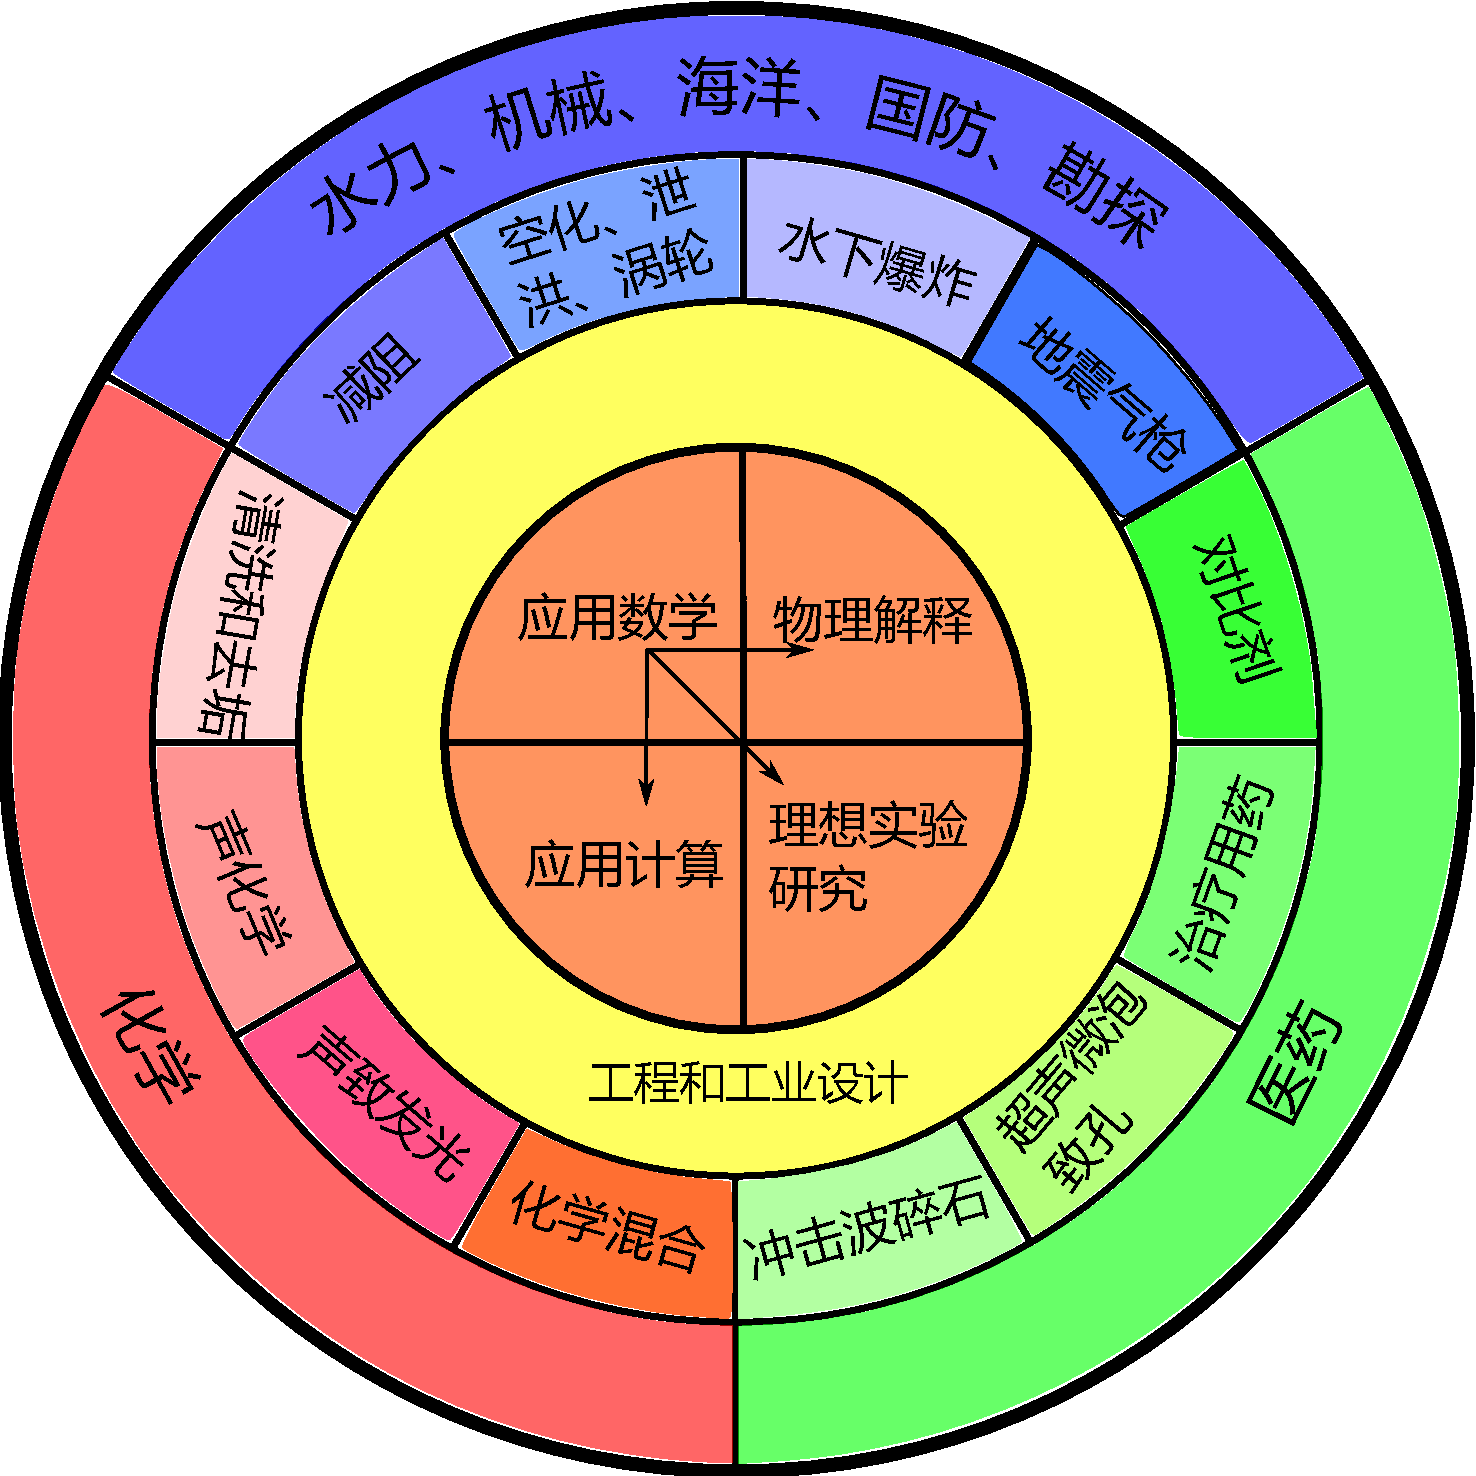
\includegraphics[bb=00 00 400 400]
{img/fig1.1.pdf}
\caption[空泡基础研究间的链接]{空泡基础研究间的链接(翻译自文献)。从理论到设计到应用的三层关系。\cite{blake_cavitation_2015}}
\label{fig1.1}
\end{figure}




空泡动力学是一个具有物理和工程意义的主题。在空泡生成的瞬间,因其位置处产生相变,相变后的气体具有极大的压强,因外界液体环境仍保持较低的原液体压强,从而使气体急剧膨胀。在这个瞬间,压力向外传导,形成一种压力间断,即空泡在诞生瞬间向外辐射一个冲击波。这个冲击波在液体环境中传播时逐渐衰减,并形成对外的力学作用。空泡受初始内部高压驱动而膨胀,直至空泡达到最大泡半径,此时空泡的内部压力为气体分压加水蒸气的饱和蒸汽压。随后空泡在外内压差驱动下而收缩。这个膨胀收缩的过程中,也会对周边形成力的作用。在空泡收缩时,其终末速度极高,形成撞击时其压力和温度可以达到非常高的程度,会向外将撞击的能量辐射出去。在空泡的球性极高时,撞击的体积及体积的表面积更小,足以形成特殊的声光效果——声致发光(sonoluminescence),甚至曾有猜测可以达到核聚变温度。人们在物理和数学层面认识了空泡动力学过程,并将其应用到了实际生产活动中\cite{Prosperetti2017}。空泡的产生方式通常采用电火花,激光,微炸药等方式激发,或者产生静态张力泡。


激光作为一种直接、高效的能量传输方式,其频率高、方向性强、能量集中,在上个世纪60年代被发明后便受到来自学界、军事和工业界的普遍而迅速的关注。随着时代的进步,高能激光与原子分子的相互作用机理逐渐清晰,激光作为能量传输载体的功能逐渐得到广泛的应用,如材料的切割、损伤、光刻,熔融成型等。激光导致的能量沉积型相变也在物理和实践中吸引了热烈的目光,特别是利用激光击穿液体的方式构建空泡,因其非接触性和极好地可控性已经成为研究空化气泡最为普遍的产生方法。短脉冲激光聚焦位置形成极高的电场强度,当其超过当地的击穿阈值时,使当地水分子发生逆韧致辐射,击穿当地液体团,并形成等离子团。这个光致电离过程涉及到多光子电离、碰撞电离、雪崩电离和隧穿电离等多个过程\cite{li__2022,__1996}。通常因为时间尺度差距较大,在研究空泡动力学时,只将其形成的等离子团在复合后的高温高压气体团作为空泡的初始阶段而不考虑其具体的击穿过程。这样就可以获得较为理想条件下的空泡动力学。同时激光强度在没有达到击穿阈值时也可以形成空泡,即利用激光的热效应,使水在当地气化即沸腾,从而形成一个高温高压的初始气泡团。通常这样的空泡多发生在界面附近,或使用长脉宽激光作为热源的情景中。

激光诱导产生的单空泡和较小数量的多空泡研究是空泡动力学研究的基石。通过理解单空泡和小数量的多空泡的运动特性,对理解空泡群体行为和将其应用具有关键的基本作用。特别地,在实际应用场景中,空泡往往不是孤立出现,而是伴随着各种约束条件,比如界面和力的作用。理解空泡在复杂力学环境内的运动是一项兼具科学和工程意义的课题。

%\section{研究现状及进展}

\section{国内外研究进展及现状}


\subsection{激光诱导击穿等离子体}
激光本质上是一种电磁波,其在一般意义上通过其电场与物质的分子原子结构进行相互作用。对于击穿中涉及的液态水的电离机制,大致可以分为强场电离与级联电离。而其中强场电离也可以分为两类:一类是束缚态电子连续吸收离散数目的光子跃迁至电离自由态的多光子电离;一类是电子隧穿通过原子库伦势与瞬态光电场的叠加势垒的隧穿电离。

1966年,G S Voronov\cite{voronov_multiphoton_1966}利用红宝石激光器辐射强电场中氙原子对气体中多光子电离展开研究,实验中发现对于在~107 V/cm 的强光场中,电离的有效性与光子束强度成正比,并且使用微扰理论的数值计算给出了电离概率的数值解。1968年,P Agostini\cite{agostini_multiphoton_1968}等人利用400MW的钕激光聚焦在一个充满惰性气体的真空室中,通过绘制离子数量与通过焦点的光束功率对比图,给出了一个原子同时吸收的光子数的数量,并且阐明了实验上光子数量的值与理论上值的差异,为后面的多光子电离研究提供了重要的理论依据。 随后,在1972年Michael\cite{bass_avalanche_1972}等人通过研究不同的材料表面损伤概率与功率密度的关系,并对这一现象进行了说明,首次提出了雪崩电离也可能是激光诱导击穿的重要原因。1981年,M. Sparks\cite{sparks_theory_1980}对固体中的电子雪崩击穿进行了理论解释,并且通过实验证明了理论的合理性的同时还获得了雪崩击穿与温度,激光脉宽,波长以及不同材料之间的依赖性,同时该理论在波长长于$1\mu m$情况下,无法正确地描述材料间的击穿现象,还必须考虑多光子吸收。

多光子电离可以分为共振跃迁和非共振跃迁两种。共振跃迁多光子电离是指原子依次吸收能量不同的数个光子,并且每个光子的能量和跃迁能级差相等,也就是原子发生跃迁时都能进入其能量本征态(即电离过程中实际的中间能级)。在实验上可以通过可调谐染料激光器激发原子实现共振跃迁多光子电离。另一种情况是原子吸收的光子能量后并未进入原子的中间能级,反而进入激光诱导的虚能级。这种跃迁不需要任何中间本征态,这通常是强激光与原子相互作用过程。由于虚能级的寿命通常很短( 或以下),所以要求激光在超短时间内产生足够的光子数才能充分激发非共振跃迁多光子电离,因此多光子电离通常需要较强的光场才能显现出来。多光子电离速率可以表示为 $W_{MPI}=\sigma_KI^k$,其中,$\sigma_K$为K个光子的电离截面,I为激光光强。

当强光场的峰值抵达原子系统时,原子的库伦势的一侧将会被明显压缩,此时电子通过右侧势垒隧穿的概率明显增加,电子波包将以一定的概率隧穿至原子势垒外侧形成电离。考虑我们现阶段研究涉及的内容,主要机制是多光子电离以及雪崩电离,此处对隧穿电离不再赘述。

当一个价带电子连续吸收离散数目的光子跃迁至边缘导带,随后通过多次逆韧致辐射机制吸收光子,从而进一步获得能量跃迁至临界导带,成为自由电子并与其他中性分子碰撞发生次级电离,额外产生一个低能的自由电子。之后,两个低能自由电子重复上述吸收光子的过程,生成四个自由电子,重复上述过程将会最终引发雪崩过程(即级联电离),造成激光汇聚区域电子数密度迅速增加,形成击穿。
相应的级联电离速率为:
$$\eta_{casc}=\frac{1}{1+(\omega\tau_c)^2} (\frac{e^2 \tau_c I}{cn\epsilon_0 \Delta Em}-\frac{m\omega^2 \tau_c}{M})\,,$$
其中,M为中性分子的质量,$\tau_c$为自由电子和分子碰撞平均所需要的时间间隔($\tau_c=1fs$),$\varepsilon_0$为真空中介电常数。在光学击穿产生等离子体的过程中,影响电子密度变化率的主要因素有:多光子电离,雪崩电离,电子的衍射扩散以及电子复合。前两个是增加电子密度的因素,后两项是减少电子密度的因素。

1995年,Kennedy\cite{kennedy_first-order_1995}将Shen\cite{shen_principles_2003}推导的简单速率方程和Keldysh\cite{fedorov_l_2016}推导的多光子电离率相结合,率先提出了在纳秒及以上脉宽层面广泛认同的,考虑了自由电子密度的全局演化的电子密度变化公式:
$$\frac{d\rho}{dt}=(\frac{d\rho}{dt})_{mpi}+\eta_{casc}\rho-g\rho-\eta_{rec}\rho^2\,,$$
其中第一项,第二项分别为多光子电离速率以及级联电离速率,已在上文中给出,对于上式中的$g$和$\eta_{rec}$分别表示的是:电子扩散出聚焦体积的速率以及电子的复合系数。对于脉宽$\tau\le10ns$时,通常会忽略扩散项$-g\rho$\cite{mlejnek_dynamic_1998,jarnac_whole_2014}且,当$\tau\le10ps$时,会将电子扩散以及复合项都忽略\cite{lenzner_femtosecond_1998,tien_short-pulse_1999}。
对于扩散项g:设光束束腰为$\omega_0$,瑞利长度为$Z_R$:$Z_R=\frac{n\pi\omega_0^2}{\lambda}$,$$
g=\frac{\tau_c\Delta E}{3m}\left[\left(\frac{2.4}{\omega_0}\right)^2+\left(\frac{1}{Z_R}\right)^2\right]\,,$$
Docchio\cite{docchio_study_1988,noack_laser-induced_1999,docchio_spatial_1991}等人通过光谱分辨测量等离子体的光衰减,获得等离子体中的复合系数的一般值:
$\eta_{rec}=2\times10^{-9}cm^3/s$。
另一种多层的电子密度演化速率方程主要用于解释皮秒以下的击穿过程,此处不述。
由于本文的重点在于空泡的动力学,故对激光致水击穿的更多详细研究过程不再赘述。


\subsection{激光致空泡动力学研究}
激光致空泡在很多领域都有诸多研究,特别是水环境下的材料处理\cite{barcikowski_materials_2019},和生物光学\cite{vogel_working_1990,juhasz_corneal_1999,toytman_multifocal_2010,jang_optothermally_2019}。通常在激光能量沉积后,形成的高能量密度高温高压的等离子体,继而演变成具有高振幅的脉动空泡\cite{47ee882c1e5b8fc9b161bae7598dafe099ccb01e},并伴随一个演化成为冲击波的压力瞬态。空泡随后运动至溃灭,并形成另外一个冲击波\cite{liang_comprehensive_2022}。等离子体的大小通常可以通过其闪光来决定\cite{vogel_shock_1996}。自由域内空泡的生存周期可以通过光偏转法,这种方法可以获得精确到nm的空泡溃灭振幅。也可以间接的通过两次冲击波的时间间隔获得,当然最简单的通过高速摄影也可以获得。但这几种获得空泡生存周期的方法的精确度逐渐递减\cite{vogel_femtosecond-laser-induced_2008,schaffer_dynamics_2002}。高球性的空泡产生通过激光的紧聚焦获得\cite{venugopalan_role_2002,obreschkow_quest_2013}。对这种理想的高球形的空泡进行物理建模,在不同精准度和不同模型考量情况下有过很多尝试。

例如Rayleigh爵士提出的解释水中的真空孔洞形成的水的运动的模型,可以一定程度上解释空泡的溃灭进程\cite{rayleigh_viii_1917}。特别是通过这个模型而获得的Rayleigh时间,也就是半程空泡生存周期,为学界所通用。其表示为
$$T_C^{Rayleigh}=0.91468R_{max}\sqrt{\rho/p_a}\,。$$

Plesset和Gilmore以及Keller等学者不断修正和添加考量量,形成了现在广为使用的Gilmore修正的Rayleigh-Plesset模型和Keller-Miksis模型\cite{Gilmore1952,plesset_collapse_1971,keller_bubble_1980,vogel_cavitation_1986,lauterborn_experimental_1975}。同时也存在着基于Rayleigh-Plesset的半经验工程模型,添加拟合常数以获得较好地拟合效果\cite{zhong_model_2020,e8c740d030b19350fce6133360d2ed165a59bd78,supponen_shock_2017,supponen_collapse_2017,obreschkow_analytical_2012,welch_pulsed_2010,selmke_bubble_2020,lohse_bubble_2018,long_early_2020}。
\bigskip
\medskip
\subsubsection{激光致空泡机制}

使用激光击穿时,激光系统的多样性,造成了空泡初始状态和后续动力学的多样性。Y.Tian和Tagawa等发现提升激光聚焦角度能极大地减小多点击穿的概率,特别是在聚焦角度大于29.8°以后,在适当的能量范围内多点击穿很少发生\cite{tian_stabilization_2016,5cc135338ea245a01dafd12d44f183533dca487e,tagawa_pressure_2016}。激光脉冲能量的提升使多点击穿的概率提升\cite{kennedy_laser-induced_1997},同时液体存在的杂质\cite{3d66d01b44fd4e7e6a8da70ed5dd2de9fca0dfac},击穿的概率发生特质\cite{kennedy_laser-induced_1997},像差\cite{evans_lens_1969,2b9cbf597962b6d717ea63693143471a76669358},等离子体的逆光生长\cite{docchio_study_1988},自聚焦\cite{potemkin_highly_2015,evans_pump-probe_2010}等都影响多点击穿的发生。多点击穿发生时,每个等离子体并不是同时发生的,而是以与焦点距离增加而变慢的\cite{docchio_study_1988, capon_nd_1988}。Evans等人\cite{evans_pump-probe_2010}发现当多个等离子体形成时,会产生多个空化气泡和冲击波。由于低密度等离子体诱导的额外气泡的形成,初始气泡和冲击波的数量有时超过等离子体的数量\cite{5a91d410705767266bdb87527d785a319238fdbf}。F.V.Potemkin等研究了透镜像差形成的长击穿和多点击穿,结果发现大数值孔径会导致击穿长度变长,进而形成更长的空泡\cite{potemkin_dynamics_nodate}。他们还利用这种长空泡产生了圆柱形冲击波前\cite{potemkin_laser_2014}。JING WANG等发现,空泡生存周期、初始冲击波远场峰值压力和相应的等离子体体积之间存在线性依赖关系\cite{fu_experimental_2018}。空泡聚合对主空泡的生存周期影响很小,但溃灭冲击波的强度和随后空泡的反弹受到很大影响,即多点击穿会抑制空泡能量转化为溃灭冲击波能量,但会增强转化为反弹空泡能量。
在多点击穿后形成的多空泡机制有可能在多个领域中发挥作用\cite{peters_highly_2013}。

关于激光击穿等离子体,也有在更复杂的激光条件和更复杂的水环境的研究。比如A. Young, 等研究了重频脉冲激光击穿水形成空泡的过程,发现激光击穿后其形成的影响在水中可以遗留达到一秒钟以上。因水中包含微泡和粒子,其会造成击穿冲击波的加强,等离子体产生位置会发生前后变动,等离子体形态也会发生改变\cite{young_laser-induced_2021}。YE TIAN,等研究深海高压环境中激光击穿产生等离子体,发现外界高压急剧减小了空泡生存周期,这使等离子体从溃灭中获得能量,提高其辐射强度,但在空泡溃灭后会立即溃灭\cite{tian_laser-induced_2020}。

当激光入射到特殊的靶材上,比如金、铂、铝等表面材料或颗粒,其光强不足以击穿水或者靶材时,这些靶材吸收光能,并转化成其内能,形成局部的过热点,从而形成沸腾机制的空泡\cite{welch_pulsed_2010,venugopalan_thermodynamic_1996,miotello_critical_1995,venugopalan_effect_1994,miotello_laser-induced_1999}。这种空泡的运动机制与击穿空泡在空泡生命周期尺度上没有差别。学界通常将他们的动力学过程混一而谈。本章中,将起归并到下文壁面附近的空泡和颗粒附近的空泡的段落中。
\medskip
\bigskip
\subsubsection{空泡的相互作用}\label{chapter1.2.2.2}

解释空泡间与各种边界相互作用时,通常会简单的采用基于势流理论推导的开尔文脉冲理论来解释\cite{Blake1987,zhang_unified_2023,blake_kelvin_1988,blake_cavitation_2015}。开尔文脉冲定义如下:
$$\bm I=\rho\int_{s}\phi ndS\,,$$
$\rho $是液体密度,$\phi$是速度势,$ S $是空泡的表面积,$n$是自液体指向气泡内部的法向模矢量。为了更加经验的简化理解空泡与其他边界条件的相互作用,还定义了一个无量纲常数:
$$\bm{\zeta} \equiv -\nabla p R_0 {\bm{\Delta}} p^{-1}\,,$$
其中的负号是为了保证射流和${\bm{\zeta}}$的方向一致。${\bm{I}}$ 和${\bm{\zeta}}$ 之间存在如下关系:
$${\bm{I}}=4.789R_0^3\sqrt{\Delta p \rho}{\bm{\zeta}}\,,$$

我们获得一个简单的用于判断各种场情况下的空泡和射流运动的参数表如下\cite{supponen_scaling_2016}:


$$\bm\zeta=-\rho \bm g R_{0} \Delta p^{-1} \quad \text { 重力场, }$$
$$\bm\zeta=-0.195 \gamma^{-2} \bm n \quad \text { 固体平面, }$$
$$\bm\zeta=+0.195 \gamma^{-2} \bm n \quad \text { 自由平面, }$$
$$\bm\zeta=-\rho(\bm u \cdot \bm \nabla) \bm u R_{0} \Delta p^{-1} \quad\text { 稳定势流, }$$
$$\bm\zeta=0.195 \gamma^{-2}\left(\rho_{1}-\rho_{2}\right)\left(\rho_{1}+\rho_{2}\right)^{-1} \boldsymbol{n} \quad\quad \text { 液体界面, }$$
$$\bm\zeta=0.195 \gamma^{-2}\left(4 \alpha-1-8 \alpha^{2} e^{2 \alpha} E_{1}(2 \alpha)\right) \bm n \quad \text { 惯性界面。 }$$

这里的$\bm u$是速度场,$\rho_x$是不同液体的密度,$\alpha$ 是一个有关密度距离和表面密度的量,$E$是一种指数积分函数。一般的,$\bm{\zeta}$可以用来判断溃灭的激烈程度和射流的方向:当$\bm \zeta\le{10}^{-3}$时,产生弱的相互作用,和弱的射流。$\bm \zeta>0.1$ 时产生强的相互作用,和强烈的射流冲击现象。中间的过渡值则产生中等程度的溃灭。
额外地,这个量还可以用来量化更多的空泡溃灭过程中存在的量:

$$ \Delta T_\mathrm{jet} / T_\mathrm{collapse}=0.15 \bm{\zeta}^{5/3}  \qquad \text{归一化的射流撞击时间}$$
$$ U_{\mathrm{jet}}/(\Delta p /\rho )^{1/2}=0.9\bm \zeta^{-1} \qquad \text{归一化的射流速度}$$
$$ \Delta z / R_0 =2.5 \bm \zeta^{3/5}\qquad \text{归一化的空泡移动距离}$$
$$V_\mathrm{impact}/V_\mathrm{max}=0.11\bm\zeta^2 \qquad \text{归一化的射流撞击时的空泡体积}$$

用来解释空泡间相互作用的理论还有也是通过势流理论和Rayleig-Plesset模型推导出的二阶Bjerknes力\cite{harkin_coupled_2001,mettin_bjerknes_1997}:
$$\langle F_1(t)\rangle=\dfrac{2\pi\rho\Omega^2R_{10}^3R_{20}^3}{D^2}\delta_1\delta_2\text{cos}(\varphi_1-\varphi_2)$$
通常其用来解释两个空泡间的吸引和排斥,此处不再详述。

\medskip
\bigskip
\subsubsection{空泡运动的模拟}

当前对空泡运动主要数值模拟方法多种多样,有基于有限体积法的VOF法\cite{lauterborn_bubble_2018,koch_numerical_2016},边界元法(BIM/BEM)\cite{klaseboer_simulations_2006,Kim2014}、格子玻尔兹曼方法(LBM)\cite{shi_numerical_2019,chen_experimental_2023,gupta_lattice_2008},光滑粒子流法(SPH)\cite{zhang_sph-bem_2019,zhang_sph_2015,wang_axisymmetric_2022},以及分子动力学(MD)\cite{shih_effect_2020},此处不再穷举\cite{ohl_shockwave_2013}。

但非常突出地,数值模拟存在一个多物理场耦合的问题,也就是通常关注空泡动力学过程的模拟研究的初值设置是经验性的。激光击穿的时间尺度通常在纳秒甚至飞秒,已有的研究能够很好的获得等离子体过程\cite{zhang_transient_2016}。在其后的等离子体分离和空泡脉动的过程因空间和时间尺度与等离子体过程差距较大。而且采用有限元方法对流体的模拟仍存在无法准确捕捉流体变形,计算量大和守恒难等问题。对两个阶段的过程的衔接仍存在着不可克服的问题。一个很有意义的尝试是赵旭宁和Kelvin Wang利用水平集和相变规则结合,将未达到击穿阈值的激光辐射用能量转化方程处理成一个脉宽热原,求解全过程的Navier-Stokes方程\cite{zhao_simulating_2023}。他们的研究能够同时且准确地描述激光辐射、气化、和后续的空泡/流体动力学过程,其计算精度达到二阶。更近一步地,基于物理辅助的机器学习的模拟方法也正在成为新的关注热点\cite{wang_machine_2021,zhai_predicting_2022,zhai_bubblenet_2022}。


\subsection{空泡受特殊力学环境影响的研究}
空泡在自然和工程应用中,往往不是孤立存在的,而是倾向于以丝、条、团簇、和云等形式存在于不同的液体环境中。下文中将以特殊环境为主题梳理空泡研究的现状。本作中将这些特殊力学环境大概的分为:多空泡间相互作用、空泡与多种界面相互作用、空泡与压力波相互作用、和空泡云及空泡成核等。
\medskip
\bigskip
\subsubsection{多空泡}
通常在多空泡的研究中,是基于一个所有空泡都独立的遵从Rayleigh-Plesset模型的假设,研究空泡群体的整体性质,但实际上,空泡往往不是独立的,而是相互影响的\cite{__2022,blake_bubble_1999,lauterborn_physics_2010,blake_acoustic_1999,Biesheuvel1984,zhang_ensemble_1994,fuster_modelling_2011,arora_effect_2007,servant_interaction_2003,johnsen_shock-induced_2008,betney_computational_2015,lauterborn_acoustic_2007}。多空泡系统中,空泡的形状、大小、生命、脉动、平移会产生不同于孤立空泡的变化。多空泡的研究可以大体分为有序排列和随机分布的两种情况。随机分布的研究,往往通过某种平均来获得多空泡间的能量集聚,空泡的侵蚀作用,空泡的噪声等。有序排列则实现简单且能具体到单个泡的动力学。泡间相互作用可以简单理解为空泡在另一个空泡的辐射声场中的运动。这种相互作用使同相的空泡相互吸引并减速溃灭,异相的相互排斥并加速溃灭。同时泡间相互作用也会改变空泡的形状,并且使空泡不均匀收缩而产生射流,由于不同距离不同相位产生的射流方向和动量也不同。多空泡场景下,空泡的最大泡半径和生存周期与孤立单空泡发生较大改变,外围和内部泡的表现也存在明显的差异。 在多空泡阵列中,相近的空泡相互改变了环境压并能够起到屏蔽作用。整个过程会持续的比孤立单空泡情况更久。通常,相比于内部空泡,边缘空泡能达到更大的尺寸,并且更快的溃灭,并且在收缩过程中形成从边缘指向内部的射流。而内部空泡在空泡阵列平面这个维度上受到相邻空泡的限制。它们的动力学演化被相邻空泡和另外的自由维度控制。 

最基础的,对多空泡的研究的开端是双空泡系统。早在1971年,Shima等人便基于球形假设研究了双空泡系统的共振频率(自然频率)\cite{shima_natural_1971}。他们发现双空泡系统自然的有两个自然频率,并且受距离和空泡大小的影响。后来Shima 还研究了双空泡系统在固体边界的运动\cite{shima_behavior_1992}。并得出固壁面会使球形空泡生存周期延长的结论。2001年,Harkin等人利用二阶Bjerkness力理论解释了双空泡的脉动和位置移动\cite{harkin_coupled_2001}。2009年Siew-Wan、Quinto-Su 、CD Ohl、B.C. Khoo等实验的研究了同相异相/同大小异大小的空泡间的相互作用\cite{fong_interactions_2009,quinto-su_interaction_2009,chew_interaction_2011}。他们总结了强、中、弱等多种相互作用强度和多种射流发生方式:同向,相向等。并用Rayleigh理论解释了泡间的相互作用。

Shen Yang 等理论的研究了双空泡系统通过声辐射相互影响而导致的理想球形空泡径向半径的变化规律\cite{shen_role_2021}。研究表明空泡能被彼此压缩或拉长,其效果取决于外界驱动声波、空泡半径、空泡距离、和空泡数目。2015年,韩冰总结以往双空泡的实验并结合Lauterborn已有研究,模拟研究了双空泡情境下的各种组合\cite{han_dynamics_2015}。反相双空泡系统中产生的射流比其他情景下都强、快、长,而且这个射流的方向是可控的。并且模拟的获得了两张关于射流速度的map图,以讨论双空泡系统参数对射流速度的影响。代表性地,国内的张阿漫、崔璞、李帅等系统地研究了双空泡系统,包括双泡系统的接合、移动、破碎、射流和冲击波激发以及变边界脉动\cite{han_experimental_2018,li_experimental_2019,wang_jet_2019,cui_experimental_2020,liu_interaction_2021}。

对双空泡系统的研究帮助展开了更进一步地多空泡相互作用的研究\cite{prigogine_experimental_2007}。多空泡往往对空泡的排布方式较为关注,一般地会形成特殊的阵列方式,如线形,面形,环形等组合。本文作者研究了三个线性对称排列的同相空泡,利用DOE三点分光镜获得等能量的激光脉冲,从而在自由水中同时地激发三空泡阵列。发现在线阵中中间空泡的多种溃灭方式,类比了空泡阵列和单空泡的溃灭逻辑,形成了对线性同相等大小空泡阵列的认知\cite{bao_experimental_2021}。后续陈荣等继续了异相线性三空泡的研究,对形成了对相位造成的射流的更多认识\cite{chen_experimental_2022}。
J.P. Dear,等在1988年通过在凝胶(gelatin)中创建静态张力泡的方法,研究了多种空泡阵列在受压力波作用后的溃灭形态,发现了屏蔽作用的存在\cite{Dear1988a,dear_study_1988}。Bremond、Ohl和Lohse等人利用壁面挖孔作为空化核,利用负压形成空泡的方法,研究了空泡阵列在壁面附近的脉动,并用Rayleigh模型和边界元方法进行了解释\cite{bremond_interaction_2006,bremond_controlled_2006}。Lauer等开发了一种界面追踪的数值算法,用来研究了冲击波对一个空泡阵列的作用。很好的验证了空泡的屏蔽,击穿和相互作用\cite{lauer_numerical_2012}。Matevz 等研究了相邻蒸汽泡对沸腾热流的影响,其通过在平板上设置多个空泡腔,并用沸腾的方法制造多空泡,发现空泡在不聚合的情况下导致的外流动只影响了较小的范围\cite{takeyama_influence_2021}。Ochiai等研究了多气泡在声压下的动力学,其溃灭表现出与空泡阵列近似的压力辐射\cite{ochiai_numerical_2017}。Tiwari等研究了一个空泡团簇在壁面附近的集体行为\cite{tiwari_growth-and-collapse_2015}。

Haiyan Chen利用二阶Bjerkness力理论解释了多空泡的脉动\cite{chen_modulation_2020}。张阿漫等也针对多空泡做了有益的探索,比如十字形和环形空泡的脉动\cite{zhang_interactions_2023}。Jian-Bo Li等研究了有不同形式排列的静态空气泡存在时的空泡溃灭强度,结果显示气泡与空化气泡相互作用的范围内,气泡与空泡的相对距离,大小和数量会极大地影响迁移方向,延长振荡时间和衰减溃灭声压,而且还产生了空泡被分裂成多个空泡的现象\cite{li_influence_2021}。秦玉鹏等理论的研究了多种空间排布空泡的动力学特性\cite{qin_analytical_2022}。Peng-li Zhang等数值的研究了更长的线性阵列组合\cite{zhang_study_2019}。多空泡的排布,内容物,边界条件的变化不一而足,此处不再详列。
\medskip
\bigskip
\subsubsection{空泡与多种界面相互作用}

空泡间的相互作用只是空泡受特殊环境影响的一个方面,更多的研究是空泡与不同形式的界面的相互作用过程\cite{Prosperetti2017,lohse_bubble_2018,lauterborn_physics_2010}。

比如空泡在水气界面,其溃灭时往往形成射向空气中的长射流,其已经获得几十年的研究\cite{boulton-stone_gas_1993,krishnan_scaling_2017,deike_dynamics_2018,e2863fbdabad074393d8ced60bcea666015f76db,6eb937979b9271fc82586961a0a59db1a3bac47c,li_bubble_2019,03a7e1892c909c181fa4619ef2eb9ea70084e02f}。因与界面的距离不同,表现出不尽相同的特性。但总的来说在膨胀时会形成液面向外的变形,并在收缩时因水的汇聚而形成射流。近期的,Juan 和CD Ohl等研究了不同曲率下的水气界面附近的空泡脉动,结果发现在靠近水气界面的空泡形成向上的射流时,同时也形成了向内的射流。这个向内的射流速度可以达到40m/s,最远可以达到15倍的空泡半径\cite{rossello_dynamics_2022}。同时在水平界面附近,这个反向射流是指向重力方向,而在曲率界面附近,张力导致的这个射流更偏向其几何中心。

同时空泡在液-液界面附近,也可以看成一种近似自由界面的动力学过程。该研究的最初动机是对液体超声(空化)制备乳液的背景有更深入的了解。Matevz等研究了液-液界面附近空泡动力学以了解界面的变形和指进,结果显示空泡产生在较轻的液体中时,空泡产生的射流将指向界面,但如果空泡产生在较稠密的液体内部,则空泡射流远离界面\cite{orthaber_cavitation_2020}。Brujan研究了空泡在gelatin附近的动力学过程,并着重的理解了杨氏模量的作用\cite{brujan_dynamics_2001}。

空泡与固体界面的相互作用因其应用广泛,是最受学界关注的方向。Blake,Brenen,Lauterborn,Prosperetti,Lohse等人都对这个主题进行了充分研究\cite{lohse_bubble_2018,lauterborn_physics_2010,blake_interaction_1993,brennen_cavitation_1995,Prosperetti2004}。
比较具有代表性的是,水下炸弹爆炸损伤船体。其过程可以大致分为三个过程:1.相变及其冲击波。冲击波相对空泡壁面具有更高的速度,在相变失去后续能量补充后的一段时间内与空泡分离。这个冲击波经水体传播后至船体,冲击波对船体形成应力损伤。2.空泡脉动。当空泡在水中持续膨胀以释放内部高压时,对固壁面形成压迫和推动。特别是在船体尺寸相对空泡尺寸不具有压倒性的尺度时,空泡的膨胀足以推动船体脱离水面。在这个过程中,因为空泡的不均匀推动和自身重力影响,会持续加重船体的应力损伤。同样的,空泡在收缩时也产生相似的机理。3.空泡溃灭冲击波和射流。空泡在完成膨胀转而收缩时,外界水体在空泡内外压差的驱动下,推动空泡收缩。由于水体的惯性,在空泡溃灭时,向外释放出水锤压力。此溃灭冲击波对船体的损伤机理类似于相变冲击波。由于在船体附近的不均匀受力,空泡在收缩时会形成指向船体的射流。此射流头部具有高速,低截面面积的特征。其可以对船体形成明显的贯穿伤害。在这个典型案例中,涉及到不同的固壁面尺寸与空泡尺寸,固壁面与空泡距离等情景,其机理涉及到空泡的推动效应和固壁面应力等。
近期地,Lechner等数值的研究了空泡在固壁面附近不同距离时形成的射流,结果显示了在不同距离下显示了两种不同的射流方式,在小距离时因空泡接触固壁面会产生特殊的针样溃灭射流,而粘度会改变这个阈值距离,同时粘度越大,射流的速度越大\cite{lechner_jet_2020,lechner_pressure_2017}。

Jia-yun Zhang等实验和数值的研究了固壁面附近激光诱导空化气泡的溃灭\cite{zhang_experimental_2022}。通过使用照明光多次曝光技术,获得空泡壁面速度。结果表明,靠近壁面的空泡溃灭成轴对称的心形,指向壁面的微射流将空化泡拉向壁面。反弹阶段产生的反射流将驱动空泡远离壁面。其中射流的速度能达到一百米每秒。

Mandeep等发现空泡的溃灭 动力学取决于其在溃灭瞬间与固壁面的接触角\cite{saini_dynamics_2022}。并通过构建正负相对距离的情景,实现了不同的接触角。当接触角小于$90^{\circ}$时,观察到的是指向墙壁的经典射流,而如果初始接触角大于$90^{\circ}$,则出现平行于墙壁的环形再入射流。这种行为的变化可以用小时间的脉冲势流理论来解释,该理论表明当接触角大于$90^{\circ}$时,在接触线的初始加速度上存在一个奇点。脉冲势流理论很好地反映了最大膨胀瞬间的空泡几何形状对整个溃灭过程的作用,该理论可以很容易地推广到其他空泡形状。

Zibo Ren等研究发现附着在固壁面表面的微纳气泡不直接响应空泡的拉伸应力,但是会被射流引起的剪切流影响而形成系链式结构,以至于分裂出更小的气泡\cite{ren_strong_2021}。
Jiayang Gu等研究了空泡冲击固壁面情况下的空泡动力学,研究了空泡与固壁面的相对距离对三种激光空化冲击(LCP)作用机制即激光冲击波,空泡溃灭冲击波和水射流的影响\cite{gu_bubble_2021}。相对距离越大,固壁面收到的冲击波强度越大,但射流越弱。他们获得了一个针对Q235钢表面硬化的最佳相对距离$\gamma=0.4$。

Jiangyou Long等使用高分辨率的频闪式阴影成像系统观察并研究了在脉冲激光烧蚀钛靶材在不同液体环境中产生的空化气泡的早期演变\cite{long_early_2020}。提出了一种流体动力学模型来计算气泡内和周围流体中的早期压力变化。结果表明,空泡是一个在初始阶段后被高压流体层所包围的低压区域,其演变主要受液体密度的影响。其演化主要受液体密度的影响。在高粘度液体中,初始气泡压力显著增加。

XiangLu等研究了空泡溃灭导致射流撞击固壁面的冲击载荷\cite{lu_equivalent_2021}。基于微射流理论和液固冲击的水锤效应,在变形等效原理下建立了单个空泡破裂微射流的冲击载荷等效模型。由于可以认为空泡均匀分布在足够小的区域内,基于单个空泡冲击载荷的等效结果,可以推导出多个空泡破裂微射流在微段内的冲击载荷等效模型溃灭微射流。形成了单个和多个近壁声泡破裂微射流空化损伤加载的等效方法。验证结果表明,这种等效冲击载荷具有极高的准确性。

Pu Cui和张阿漫等研究了利用空泡溃灭的破冰的研究,包括单空泡和双空泡的情景\cite{cui_experimental_2020,cui_ice_2018}。当单空泡作用时,冰板从顶部诞生裂缝,即从冰-空气界面发展。这归因于冲击波在界面上的反射引起的张力。当冰板的厚度或空泡-冰的距离增加时,这种断裂会减弱。当空泡-冰的距离足够小时,在冲击波入射时也可能从冰板底部形成断裂。空泡形变和冲击波也能推动冰板的运动。双空泡作用时,观察到独特的空泡行为,包括合并、分裂、倾斜的反射流和不对称的环形空泡溃灭。测量了研究了空泡动态特性,例如射流速度、射流能量和气泡中心位移。在一系列空泡间和空泡-边界距离情境下,使用压力换能器测量了两个空泡的冲击波辐射,表征了其破冰能力。他们发现在多种组合的情况下,通常在冲击波减弱时其损伤效果会同步的减弱。Gregorčič等还研究了空泡在固体边界和自由界面间的动力学\cite{Gregorcic2007}。讨论了生存周期受自由界面缩短和硬边界延长的两种效应。

在更工程的层面理解空泡与固壁面的相互作用,自然而然的会谈到空泡的侵蚀和清洗作用。Fabian和CD Ohl揭示了在空化气泡的非球形坍塌过程中导致能量集中并最终导致硬化金属腐蚀的决定性机制\cite{reuter_cavitation_2022}。研究表明,只有在非轴对称的能量自聚焦情况下,接近金属表面的环境压力下的单个空泡才会引起侵蚀。空泡在溃灭时首先在一点汇聚,并产生冲击波,其他残余气体形成被这个冲击波强化的溃灭。同时他们还证明了只有在相对距离足够小时($\gamma<0.2$),硬质表面才会产生侵蚀。常规射流即使达到100m/s,也没有造成损伤,因此他们建议,在需要考虑减小损伤的情况下,空泡形成射流时要同步破碎,以防止产生针状射流和不对称自聚焦。反之也可以加强损伤。Fabian等人开发了一种利用空泡损伤铝制材料表面氧化膜形成的导电性能变化来计量空泡损伤效果的方法,这种方法具有以微秒分辨率,非侵入性、就地实时的优点\cite{abedini_situ_2023}。其在靠近铝样品表面的 NaCl 水溶液中产生单个激光诱导气泡。高速计时电流法用于记录样品和浸入相同溶液中的相同铝电极之间流动的腐蚀电流。这种配置使得可以通过再钝化产生的腐蚀电流来测量铝表面纳米薄钝化层中的空化损伤。与腐蚀电流与同步的高速成像记录之间的相关性允许对空泡动态的各个阶段造成空化损坏进行计量。对于最小的初始相对间距,观察到最大的空化感应电流。随着空泡在几个阶段中重新膨胀和再次破裂,检测到更多的电流峰值,这意味着一系列较小的损坏。在中间距离处,空泡不会造成破坏,而在较大的距离处,空泡只会在第二次发生在固体表面的溃灭期间造成破坏。Park等对比了气体泡和水蒸气泡在超声场的驱动下对硬质表面的清洗效果\cite{park_comparing_2021}。研究发现气体和蒸汽空泡在超声场中表现出不同的动态行为,蒸汽空泡和气泡分别能更有效地去除附着力强和弱的污染物,此外,蒸汽空泡能更好地清洁疏水性基材。

激光照射材料靶材,其形成的纳米级材料喷溅,是当前生产纳米粒子的一种通用方法。在这个过程中产生的空泡和粒子的相互作用也引起了很多兴趣。特别是人们发现,可以利用空泡来驱动粒子实现特定的运动时,许多研究者对激光与颗粒的相互作用的过程进行了研究。

Liang Lv和Yuning Zhang等实验研究了空泡与颗粒距离对近似大小的空泡与悬挂颗粒相互作用的影响\cite{lv_experimental_2019}。研究发现近距离排斥和远距离吸引的机制。远距离吸引可以用辐射压力来解释。近距离排斥则可以用射流来解释。Xiaoyu Wang 和Yuning Zhang实验的研究了球形粒子附近的激光诱导空泡的动力学\cite{wang_theoretical_2022}。并用Weiss定理获得了开尔文脉冲理论模型。他们发现只有在相对距离γ>0.5时,空泡能较好的保持球形时才能使用开尔文脉冲模型解释空泡行为。颗粒对空泡与颗粒之间液体流速的影响主要受几何上空泡在颗粒的镜像位置影响,这块区域的液速总是低于周围其他区域。而空泡的中心移动可以用开尔文脉冲预测,并宣称了一个所谓的常数来获得开尔文脉冲与速度的线性关系。同一团队的Xiaoxiao Zheng 则实验的研究了两个相同尺寸的球形颗粒附近的空泡动力学\cite{zheng_investigation_2023}。他们认为开尔文脉冲理论模型能够有效地预测两个相同尺寸粒子附近的空泡的运动特性。当空泡初始位置沿水平对称轴逐渐远离两个大小相同的粒子附近的粒子时,第一周期空泡质心的移动距离先增大后减小。当空泡质心的初始位置在两个粒子附近的不对称位置时,空泡质心的运动方向偏向离空泡较近的粒子,而不是偏向该粒子的中心。

Linglong Wang等用高速全息显微术对激光诱导空泡进行了成像研究\cite{wang_measurement_2021}。他们发现不同尺寸的纳米空泡的脉动具有细微的差别。这种差别在归一化并平方后显示出与空泡半径的相关性。其结果表明,空泡的半径越大,脉动的进程越快。这是由空泡传热过程改变引起的。

Matevz同样研究了空泡在球形颗粒附近的动力学,以期解释微纳空泡杀菌的作用\cite{zevnik_cavitation_2022,zevnik_cavitation_2020}。结果中讨论了射流、冲击波、剪切力和热效应。并考虑到表面张力在小尺度上会引起的射流减弱效应。球形颗粒上的机械载荷倾向于随着球形-气泡尺寸比的增加而增加,并随着它们的距离增加而减少。他们还给出在溃灭末期,空泡对颗粒的压力影响可以达到$100 MPa /\mu m$的梯度。

Chunhui Luo  等研究发现利用激光空泡降解悬浮液有机物时,激光能量的提升对降解效果的提升在一定范围内是线性的,但在能量过高后等离子体的吸收效应会限制空泡生长,导致其有一个平顶式增长。同时发现,固体颗粒物在超过一定范围后浓度越大,激光空泡形成的溃灭效应越弱\cite{luo_impact_2021}。而且在固体边界附近中的空泡降解效果更好。其原因作者没有探讨,但其理所当然的来自更剧烈地非对称溃灭形式的自我强化。

Shengji Wu和刘树红研究了在固体界面附近产生的激光空泡驱动球形粒子的动力学\cite{wu_dynamics_2021}。结果发现了当颗粒在远离固体界面和空泡端时,颗粒的移动主要受空泡膨胀的影响。当颗粒在空泡和界面之间时,颗粒的移动呈现出多种方式。但最主要的当粒子距离空泡足够近时,空泡膨胀才会推动粒子撞击固体表面。当颗粒恰好在空泡正下方时,即使空泡在膨胀时没有接触到颗粒,颗粒也会被射流加速到多倍于空泡膨胀推动的速度。

Sieber和Farhat等研究了在固体界面上布置了纳米颗粒的情景下,空泡与其相互作用的过程\cite{sieber_dynamics_2022}。结果显示当相对间距γ>1.3时,该动力学表现为空泡与固体边界的相互作用机制。当0.6<γ<1.3时,空泡在溃灭时会将颗粒举起并形成一个小堆,这个小堆的尺寸取决于空泡与颗粒的相对尺寸和相对间距。在相对间距足够小时,空泡在溃灭时会形成钟型图样,并形成一个微射流。但在所有案例中,空泡的生存周期都因为泡能用来驱动纳米颗粒而消耗,从而形成生存周期的缩短。

因为空泡在自然界中和工程应用中涉及到的环境情况多种多样,学者们关心和关注到的现象和潜在的场景也多种多样。于是,更复杂的空泡与环境的相互作用场景也不胜枚举,下面仅述几例复杂边界的研究。

Brujan等研究了激光空泡在相互垂直的两个固体壁面间的动力学。结果表明,这种空泡的行为及其依赖于泡沫与墙壁之间的距离\cite{brujan_dynamics_2018}。当空泡溃灭时,会形成一个倾斜的射流,射流指向更偏向距离更近的壁面,当距离相等时则指向中间。且空泡会朝着射流方向移动。而射流击穿空泡后,空泡形成环状结构。这个结构在里壁面较远时,沿着径向溃灭形成小空泡。当这个环状结构接触到壁面时,接触部分会沿着壁面迁移并首先溃灭。从而形成新月状残余。

Yoshiyuki Tagawa等研究了水气自由面和垂直固壁面附近的空泡\cite{kiyama_direction_2021}。通过理论预测和实验验证,成功的给出了一个射流倾角关于相对位置的模型。

Abboud研究了在一个固体壁面上的孔洞结构对激光空泡动力学的影响\cite{abboud_microjetting_2013}。研究表明,即使在存在孔洞的情况下,空泡仍形成了一个指向固壁面所在平面的射流,并且这个射流会通过这个孔洞。一般地,空泡膨胀会在通孔处形成快速流动,并产生次级空化。在空泡膨胀通过孔洞后,在收缩时,凸出的灯泡状结构会脱落形成小空泡,在溃灭时形成朝向主空泡的反射流。

Hendrik和CD Ohl等研究了激光空泡在固壁面上通孔上方时的动力学过程\cite{reese_microscopic_2022}。针对通孔的长度,宽度和形状,以及空泡的尺寸,液体的粘度,空泡与壁面的距离,做了具体的研究。研究发现了三种射流机制,正向,反向,以及针形射流。

利用空泡形成乳化液滴也是一个非常常见的应用\cite{raman_microemulsification_2022,nieves_ultrasound-assisted_2021}。空泡是乳液形成的重要机制。空泡取决于油滴的粘性而形成不同的喷溅状态。

Xianmei Zhang等研究了在液滴内形成的空泡的脉动和位置移动\cite{zhang_radial_2022}。他们通过将体积模量考虑进状态方程推导出一个液滴内空泡脉动的类Rayleigh-Plesset方程,并据此研究了这个空泡的径向脉动和位置移动,他们把形成这种特殊平动的机制归因于液滴表面的限制。

Jingzhu Wang等研究了夹在两个薄板间的液滴内的空泡引起的液滴Rayleigh–Taylor不稳定性\cite{wang_rayleightaylor_2021}。实验、理论和数值模拟都获得了三种独立液滴形态:喷溅、贯通、和稳定状态。并通过定义了两个参数来研究了这三种状态。而空泡第一次溃灭形成的射流方向,取决于液滴与空气界面的接触角。

Zhao Fang等人还研究了利用空泡形成的微射流将固体颗粒表面的油滴去除\cite{zhao_numerical_2021}。通常大空泡的对大团油滴的清洗效果较好,而小空泡则对狭小局部的油滴的去除效果好。

Jin-Jie Deng等研究了在静电场与超声场中耦合作用下的空泡脉动\cite{deng_dynamics_2021}。研究发现静电场中的空化阈值更低。电应力降低了表面张力,导致空泡趋于不稳定而加速溃灭。但同时也提高了最大泡半径也降低了最小泡半径。有电场存在的情况下,空泡的动力学更加剧烈。

Tomaˇz Poˇzar等研究了一个模拟眼球形状下的激光击穿空泡\cite{pozar_laser-induced_2021}。也就是在一个凹面结构附近形成激光击穿。激光冲击波和溃灭冲击波通过反射,在焦点处形成次级空泡。

Matej Senegac ˇnik等设计了一个悬崖式固体壁面,悬崖是一个直角,并将这个固体结构浸没在不同的液体介质中,而空泡在悬崖表面产生\cite{senegacnik_dynamics_2021}。研究显示,空泡快速膨胀形成的高速水流在悬崖外侧形成次级空化,并在空泡边缘到达悬崖边缘时,形成涡流再次进入空泡内部。提高液体粘度,可以防止这种再入。

Yuning Zhang 等也研究了这种悬崖式表面,但他们将空泡放置在角平分线的反向延长线上,而不是表面\cite{zhang_collapsing_2020}。研究发现,这种结构能够明显的延长空泡生存周期。当空泡距离角顶点较近时,空泡收到束腰式限制。但距离中等时,空泡溃灭时将形成橄榄状,并且向角顶点移动。

Qingyun Zeng和CD Ohl研究了由两个刚性壁为边界的薄液隙中的激光空泡和诱导射流的动力学\cite{zeng_splitting_2020}。研究发现液隙的相对高度和空泡处于液隙的相对位置,对空泡的动力学表现具有决定作用。他们发现了三种射流形式:空泡分裂后射向两边,直接射向最近的壁面,和射向远端壁面的转换射流。特别地,这种转换射流是因为空泡相对液隙足够大,在膨胀面接触远端壁面后形成的射流方向转换。只存在于某些极端情况,这个机制决定于液体粘性边界层。
空化在牛顿流体中得到了广泛的研究,在剪切稀化流体中的研究程度较低但很重要。Guillaume T. Bokman和Outi Supponen研究了水-玉米淀粉悬浮液这种剪切增稠流体中的空泡动力学\cite{bokman_cavitation_2022}。这种流体的一个有趣特性是,当应变率增加时,它们的粘度会增加,直到它们表现出类似固体的行为,甚至会破裂。由于空泡能够产生极端应变率,其受到剪切增稠流体行为的影响。文章用Keller-Miksis 方程解释了其行为。在实验过程中也观察到了空泡膨胀导致的液体的碎裂。

空泡与生物组织的研究,多利用不同浓度的凝胶Gelatine代替生物组织。

Kodama等研究了空泡在水-凝胶(water-Gelatine)边界附近的脉动\cite{kodama_cavitation_2000}。空泡倾向于向界面移动但不会产生射流。空泡的生存时间除了在小相对距离情况下,其他情况都被延长。但在凝胶内部可以检测到10Mpa以上的压力。Oguri等研究了激光致冲击波与空泡相互作用在凝胶里导致的次级空化现象\cite{oguri_cavitation_2018}。得出凝胶中的起始空化阈值约为-24Mpa,与水中差别不大。

Dui Qin 等研究了空泡在生物组织中的动力学和声辐射\cite{qin_nonlinear_2021}。他们通过数值地研究粘弹性组织中两个相互作用的空化气泡的径向和平移运动以及由此产生的声发射,发现在他们文章的条件下双空泡对大空泡的增强作用。随着距离的增加,抑制逐渐减小,其辐射声波出现谐波、次谐波、超谐波和宽带分量的逐步演变。随着周围介质弹性和/或粘度的增加,气泡的非线性动力学和平移运动均显着降低。郎骥和吴千红等研究了空泡导致脑损伤的过程\cite{lang_cavitation_2021}。在这项研究中,用人造透明头部替代物发现了当头部受到突然的平移冲击时,撞击位置突变引起空泡的形成和溃灭。他们发现,空泡在脉动过程中对大脑表面形成损伤,并向大脑内部传播冲击波。对大脑内部形成暗损伤。
\medskip
\bigskip
\subsubsection{空泡与压力波相互作用}


Blake 等研究了行波驻波对空泡的影响\cite{wang_non-spherical_2010,wang_non-spherical_2011}。他们推导声扰动对空泡壁的作用到二阶解。发现空泡中心压强和振荡辐射压强导致了球面波行为,声波导致的惯性行为导致非球面波行为。气泡的形状在弱声波时,可以维持球形。当空泡的自然频率等于声波频率时,空泡会一直吸收声波能量,而振幅逐渐扩大,半径极大值更大,极小值更小。在强声波时,一般会形成沿着声波方向的射流击穿。在驻波场内时,Bjerkness力导致了非球形效应,其与声波频率平方成正比,同时这个力还导致了空泡的平移和非球形变形。当低频时,空泡在整个流场中保持近似球形,并会移动到声波波腹位置。高频时。空泡在Bjerkness力消失的波腹保持球形。在波节和波腹之间的空泡则会朝着波节移动,并在溃灭时失去球形,其射流也指向波节。

Pei Zhong等研究了冲击波对空泡动力学的影响\cite{klaseboer_interaction_2007, sankin_shock_2005}。他们发现了冲击波对空泡的强制溃灭。空泡在膨胀期收到作用,在继续膨胀一段时间后被强制溃灭。在收缩其收到作用后,迅速强制溃灭。所以在溃灭期的收到作用的空泡溃灭时间最早。而在稳定期收到作用时,因空泡半径足够大,从而被强制溃灭的时间最晚。

Jing Luo 和BC Khoo研究了激光空泡的冲击波过程与附近气泡的相互作用\cite{luo_stratification_2021}。他们发现在相对距离大于一个关于尺寸的线性函数值时,气泡对空泡的溃灭影响极小。当小于这个值时,空泡水锤和内爆冲击波产生时空延迟,从而显示出冲击波的分层。当距离更近的时候,空泡和气泡合并,也会产生冲击波分层。在冲击波显示分层时,这些波的强度至少衰减了40\%。

Ma Yan等\cite{ma_nonlinear_2021}利用气泡的散射理论研究了气泡的非线性振荡和球形空泡团簇的散射声场。在空泡团簇的不同位置,空泡的振荡相位有一定程度的延迟,但在不同位置,空泡的振荡半径没有太大的差异。此外,空泡的声散射的方向性是明显的。在空泡簇内部和外部的不同位置,散射声压不同。球形气泡簇的散射声场取决于驱动压力幅度,驱动频率,空泡的平衡半径,空泡数和球形气泡簇的半径。

Hao Wu等研究了声场中固壁面附近的空泡动力学\cite{wu_effects_2021,wu_experimental_2020}。研究发现低表面张力降低了气泡在液体介质中的稳定性。在表面张力较低的液体中,空泡平移更加显著,在平移过程中会更早距离壁面更远的位置溃灭。表面张力对第一次微射流的速度没有显着影响,但可以在气泡第一次破灭后大幅度提高第二次和第三次微射流的速度。

Xiao Huang等研究了超声驻波场内固壁面附近的空泡对的动力学\cite{huang_nonlinear_2020}。研究发现考虑粘性的条件下,低频声场会产生更强的空泡溃灭,竖直排列在表面上的空泡对形成射向表面的溃灭射流更加强烈,而不同尺寸的竖直排列空泡则显示出更强的射流。

Tanguay等研究了冲击波和空泡云的相互作用\cite{tanguay_computation_2004}。提出了空泡云对冲击波能量的储存和释放机制。在空泡的膨胀期,云中心的压力略小于环境压。在溃灭期,流体相向空泡云中心挤压,并形成巨大的压力升高,可以将没有云相互作用机制下的空泡溃灭能量提高一个数量级。
\bigskip
\subsubsection{空泡云及空泡成核}

激光空泡与冲击波的相互作用研究中,往往不可避免的现象就是空泡云现象的发生。而且实际上,空泡在更多范围内存在形式是以空泡云形式存在的。空泡云的研究涉及到了空化核和压力赋能等研究。

Biasiori-Poulanges和Olivier Coutier-Delgosh等利用高速同步辐射X-ray相衬成像观察了空泡云的形成和运动\cite{biasiori-poulanges_synchrotron_2023,zhang_experimental_2020}。研究发现空泡云的形成分成多个阶段,即从一个空泡脉动到多空泡云的过程。

Matheus Andrade等研究了空化核的成长过程\cite{DEANDRADE2022106091}。通过量化压力和温度对成核的相对优势,设置了多个无量纲数研究了粘度、惯性、表面张力和蒸汽传输对空泡成长的影响。粘性效应在 0-120°C 温度范围内控制着类水介质中的超声成核过程,尽管这种优势随着温度的升高而降低。焓传递降低了温度升高的成核率。这种效应在高于 30 °C 的温度下变得显着,并有利于产生更少的更大尺寸的原子核。相反,在较低温度下可忽略的焓传输可以使密集的小核团簇成核,例如空化云

Hong等研究了水的空化阈值问题\cite{hong_numerical_2022}。结果显示声频率和空化核尺寸的变大能够极大的减小空化阈值。并拟合了一个声空化的阈值函数。

Juan和CD Ohl通过建立冲击波和未击穿激光相互作用的实验装置,认为水中存在纳米级尺寸的空泡,并基于流体力学的将这个结论推广到普适\cite{rossello_-demand_2021}。他们通过这种方法能够在特定区域,即激光路径和冲击波路径结合处获得大块纳米空泡团。并对这个空泡团的特性比如对声脉冲的响应和其生存时间进行了评估。但实际上该研究忽略了激光的入射形成的局部汽化效应,而只是将之归因于水天然的存在纳米空泡。

Pan Zhao等人通过撞击产生冲击波,并以此在水中产生大空泡或者空化云 \cite{speirs_cavitation_2021,xu_criteria_2021,pan_cavitation_2017}。

Pflieger等研究了含不同内容气体的空泡在超声场内稳定存在的半径\cite{pflieger_impact_2021}。

姚熊亮等研究了空化成核理论,并通过实验发现压降后,空化核的整体数密度提升,但大核数密度降低\cite{yao_study_2020}。



\section{主要内容及章节安排}
本文的目的在于尝试以实验和模拟的方法探究几种复杂力学条件下激光致空泡与水环境的相互作用的动力学机理,提出潜在的工程应用可能。
第二章中,对实验方法和数值方法进行了简单的介绍。
第三章中,集中的利用OpenFOAM框架下的求解器下求解液-气、液-液、液-固界面附近的空泡脉动,解释了空泡的溃灭形态及射流的形成。
第四章中,研究了准自由域中,激光激发的同相等大小空泡线性阵列的动力学。 利用实验和模拟集中讨论了三个同相空泡在统一的不同间距的排布,在空泡的初生到溃灭过程中的变形、尺寸、生存周期、和移动。
第五章中,探索了激光空泡在试管受限域内,受脉冲压力波的作用下的动力学。其中,空泡在自由下落的液体试管中产生。通过控制试管与平台的撞击时间,使得我们能够分析空泡在遭受到冲击正压波或反射后的舒张波时暴露出来的动力学行为。此外,我们还将其与容器停止运动时的静态环境下的空泡与其自由落体时的的空泡动力学进行了对比。



